\title{Nonparametric Goodness-of-Fit Tests for Discrete Null Distributions}
\author{by Taylor B. Arnold and John W. Emerson}

\maketitle

\abstract{
Methodology extending nonparametric goodness-of-fit tests
to discrete null distributions has existed
for several decades. However, modern statistical software
has generally failed to provide this methodology
to users. We offer a revision of R's \code{ks.test()} function
and a new \code{cvm.test()} function that fill this need
in the R language for two of the most popular nonparametric
goodness-of-fit tests. This paper describes these contributions and
provides examples of their usage. Particular attention is given
to various numerical issues that arise in their implementation.
}

\section{Introduction}

Goodness-of-fit tests are used to assess whether data are consistent
with a hypothesized null distribution.  The $\chi^2$ test is the best-known
parametric goodness-of-fit test, while the most popular nonparametric tests
are the classic test proposed by Kolmogorov and Smirnov followed closely by
several variants on Cram\'{e}r-von Mises tests.

In their most basic forms, these nonparametric goodness-of-fit
tests are intended for continuous hypothesized distributions, but they have
also been adapted for discrete distributions.  Unfortunately,
most modern statistical software packages and programming environments
have failed to incorporate these discrete versions.  As a result,
researchers would typically rely upon the $\chi^2$ test or
a nonparametric test designed for a continuous null distribution.
For smaller sample sizes, in particular, both of these choices can produce
misleading inferences.

This paper presents a revision of R's
\code{ks.test()} function and a new \code{cvm.test()} function to
fill this void for researchers and practitioners in the R environment. This
work was motivated by the need for such goodness-of-fit testing in a study
of Olympic figure skating scoring \citep{emersonarnold2010}.  
We first present overviews of the theory and general implementation of the
discrete Kolmogorov-Smirnov and Cram\'{e}r-von Mises tests.  We discuss
the particular implementation of the tests in R and provide examples.  We
conclude with a short discussion, including the state of existing continuous
and two-sample Cram\'{e}r-von Mises testing in R.

\section{Kolmogorov-Smirnov Test}

\subsection{Overview}

The most popular nonparametric goodness-of-fit test is the
Kolmogorov-Smirnov test.
Given the cumulative distribution
function $F_0(x)$ of the hypothesized distribution
and the empirical distribution function $F_{data}(x)$ of the
observed data,  the test statistic is given by
\begin{align}
D = \sup_x \left| F_0(x)- F_{data}(x) \right|.    \label{eqD}
\end{align}
When $F_0$ is continuous, 
the distribution of $D$ does not depend on the hypothesized
distribution, making this a computationally
attractive method. \cite{slakter1965} offers a standard presentation
of the test and its
performance relative to other algorithms. 
The test statistic is easily adapted for one-sided tests.
For these, the absolute value in (\ref{eqD}) is discarded and the tests are based
on either the supremum of the remaining difference (the `greater' testing
alternative) or by replacing the supremum with a negative infimum
(the `lesser' hypothesis alternative).  Tabulated $p$-values have been
available for these tests since 1933 \citep{kol33}.

The extension of the Kolmogorov-Smirnov test to non-continuous 
null distributions is not straightforward. The formula of
the test statistic $D$ remains unchanged, but its distribution
is much more difficult to obtain; unlike the 
continuous case, it depends on the null model.
Use of the tables associated
with continuous hypothesized distributions results in conservative $p$-values
when the null distribution is discontinuous 
(see \cite{slakter1965}, \cite{goodman1954}, and \cite{massey1951}).  
In the early 1970's, 
\citet{Conover1972} developed the method implemented here
for computing exact one-sided $p$-values
in the case of discrete null distributions.
The method developed in \citet{gleser85} is used provide exact p-values
for two-sided tests.

\subsection{Implementation}

The implementation of the discrete Kolmogorov-Smirnov test involves
two steps. First, the particular test statistic is calculated
(corresponding to the desired one-sided or two-sided test).
Then, the $p$-value for that particular test statistic may be computed. 

The form of the test statistic is the same as in the
continuous case; it would seem that no additional work would be required
for the implemenetation, but this is not the case.
Consider two non-decreasing functions $f$ and $g$, where the function $f$ is a step function with jumps on the set $\{x_1, \ldots x_N \}$ and $g$
is continuous (the classical Kolmogorov-Smirnov situation).
In order to determine the supremum of the difference between
these two functions, notice that
\begin{align}
\sup_x \left| f(x) - g(x) \right| &  \nonumber  \\
       =  \max_i \bigg[ \max\bigg(  & \left|g(x_i) - f(x_i) \right|, \nonumber \\
& \lim_{x \rightarrow x_i} \left| g(x) - f(x_{i-1})
   \right| \bigg) \bigg] \label{SUP1}\\
=  \max_i \bigg[\max \bigg( & \left|g(x_i) - f(x_i) \right|, \nonumber \\
& \left| g(x_i) - f(x_{i-1}) \right| \bigg) \bigg]. \label{SUP2}
\end{align}
Computing the maximum over these $2N$
values (with $f$ equal to
$F_{data}(x)$ and $g$ equal to $F_0(x)$ as defined above) is clearly the 
most efficient way to compute the Kolmogorov-Smirnov test statistic for
a continuous null distribution. When the function $g$ is not
continuous, however, equality (\ref{SUP2}) does not hold in general because 
we cannot replace $\lim_{x\rightarrow x_i} g(x)$ with the value $g(x_i)$. 

If it is known that $g$ is a step function, it follows that
for some small $\epsilon$,
\begin{align}
\sup_x &\left| f(x)- g(x) \right| =  \nonumber \\
        & \max_i \left( \left|g(x_i) - f(x_i) \right|, 
    \left| g(x_i - \epsilon) - f(x_{i-1}) \right| \right) \label{epsilon}
\end{align}
where the discontinuities in $g$ are more than some distance $\epsilon$ apart. 
This, however, requires knowledge that $g$ is a step function as well as of
the nature of its support (specifically, the break-points).  As a result,
we implement the Kolmogorov-Smirnov test statistic for discrete null
distributions by requiring the complete specification of the null distribution.

Having obtained the test statistic, the $p$-value must then be calculated. 
When an exact $p$-value is required for
smaller sample sizes, the methodology in \citet{Conover1972} is used in
for one-sided tests.  For two-sided tests, the methods presented in
\citet{gleser85} lead to exact two-sided $p$-values.  This requires the
calculation of rectangular probabilities for uniform order statistics
as discussed by \citet{nieder81}.
Full details of the calculations are contained in source code
of our revised function \code{ks.test()} and in the papers of
Conover and Gleser.  

For larger sample sizes (or when requested for smaller sample sizes),
the classical Kolmogorov-Smirnov test is used
and is known to produce conservative p-values for discrete distributions;
the revised \code{ks.test()} supports estimation
of p-values via simulation if desired.


\section{Cram\'{e}r-von Mises Tests}

NOTE: NEED TO ADD SIMUALTED P-VALUES.

\subsection{Overview}

While the Kolmogorov-Smirnov test may be the most popular of
the nonparametric goodness-of-fit tests, Cram\'{e}r-von Mises
tests have been shown to be more powerful against a large class
of alternatives hypotheses. 
The original test was developed by
Harald Cram\'{e}r and Richard von Mises \citep{cramer1928, vonmises1928} 
and further adapted by \cite{anderson1952}, and  \cite{Watson1961}. 
The original test statistic, $W^2$, Anderson's $A^2$, and Watson's
$U^2$ are:
\begin{align}
W^2 &= n \cdot \int_{-\infty}^{\infty} \left[ F_{data}(x)- F_{0}(x) \right]^2 dF_0(x) \label{W2} \\
A^2 &= n \cdot \int_{-\infty}^{\infty} \frac{\left[F_{data}(x)- F_{0}(x) \right]^2}{F_0(x) -F_0(x)^2} dF_0(x) \label{A2} \\
U^2 &= n \cdot \int_{-\infty}^{\infty} \left[ F_{data}(x)- F_{0}(x) - W^2 \right]^2 dF_0(x) \label{U2}
\end{align}
As with the original Kolmogorov-Smirnov test statistic, these all have 
test statistic null distributions which are independent of the
hypothesized continuous models.
The $W^2$ statistic was the original test statistic.
The $A^2$ statistic was developed by
Anderson in the process of generalizing the test for the two-sample case.
Watson's $U^2$ statistic was developed for distributions
which are cyclic (with an ordering to the support but
no natural starting point); it is invariant to cyclic reordering of
the support.   For example, a distribution on the months of the year
could be considered cyclic.

It has been shown that these tests can be more powerful than 
Kolmogorov-Smirnov tests to certain deviations from the hypothesized distribution. 
They all involve integration over the whole range of data, rather than
use of a supremum, so they are best-suited for situations where the
true alternative distribution deviates a little over the whole support
rather than having large deviations over a small section of the support. 
\cite{stephens1974} offers a comprehensive analysis of the relative powers
of these tests.

Generalizations of the Cram\'{e}r-von Mises tests to discrete
distributions were developed in \cite{choulakian1994}. As with the
Kolmogorov-Smirnov test, the forms of the test statistics are unchanged, 
and the null distributions of the test statistics are again hypothesis-dependent. \cite{choulakian1994} does not offer finite-sample results, but rather 
shows that the asymptotic distributions of the test statistics under the null hypothesis each involve consideration of a weighted sum of independent
chi-squared variables (with the weights depending on the particular
null distribution). 

\subsection{Implementation}

Calculation of the three test statistics is done using the
matrix algebra given by \cite{choulakian1994}. 
The only notable difficulty in the implementation of the discrete form
of the tests involves calculating the percentiles
of the weighted sum of chi-squares,
\begin{align}
Q = \sum_{i=1}^{p} \lambda_i \chi^2_{i,1df},   \label{eqQ}
\end{align}
where $p$ is the number of elements in the support of the hypothesized
distribution.
\cite{imhof1961} provides a method for obtaining the distribution of $Q$,
easily adapted for our case because
the chi-squared variables have only one degree of freedom.
The exact formula given for the distribution function of $Q$
is given by
\begin{align}
\mathbb{P}\{Q \geq x \} = \frac{1}{2} + 
\frac{1}{\pi} \int_{0}^{\infty} \frac{\sin\theta(u,x)}{u \rho(u) } du \label{distQ}
\end{align}
for continuous functions $\theta(\cdot, x)$ and $\rho(\cdot)$ depending on the  weights $\lambda_i$. 

There is no analytic solution to the integral in (\ref{distQ}), 
so the integration is
accomplished numerically. This seems fine in most situations we considered,
but numerical issues appear in the regime of large test statistics $x$
(or, equivalently, small $p$-values).
The function $\theta(\cdot, x)$ is linear in $x$; as the test statistic 
grows the corresponding periodicity of the integrand decreases and
the approximation becomes unstable. 
As an example of this numerical instability, the red plotted in
Figure \ref{cvmissues} shows the non-monotonicity of the numerical
evaluation of equation (\ref{distQ}) for a null distribution that is
uniform on the set $\{1,2,3\}$.

\begin{figure}
\begin{center}
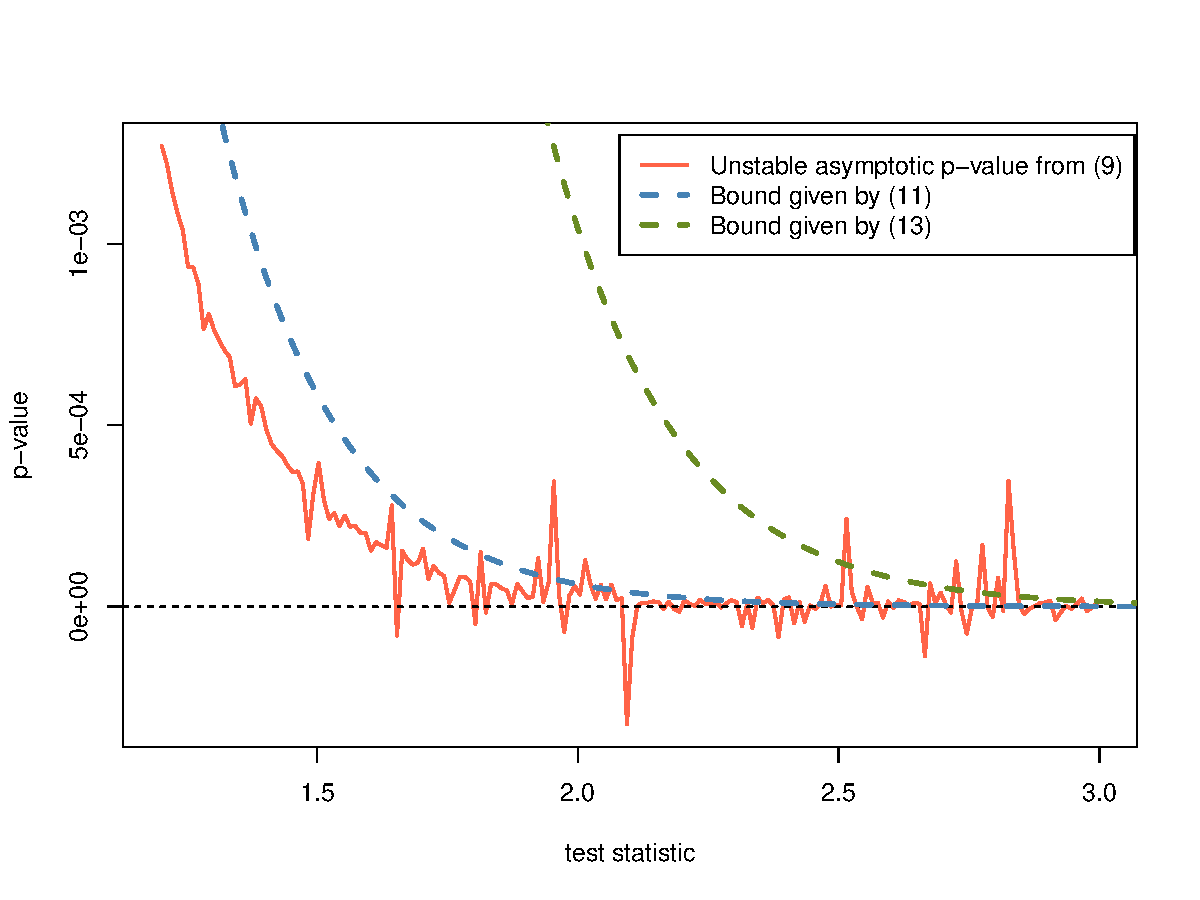
\includegraphics[scale=0.4]{fig1.pdf}
\end{center}
\caption{Plot of calculated $p$-values for given test statistics
using numerical integration
(red) compared to the conservative chi-squared bound (dashed blue) and
the Markov inequality bound (dashed green). 
The null distribution is uniform on the set $\{1,2,3\}$ in this example.
The sharp variations in the calculated $p$-values are a result of numerical
instabilities, and the true $p$-values are bounded by the dashed curves.}
\label{cvmissues}
\end{figure}

We resolve this problem by using a combination of
two simple conservative approximations to
avoid the numerical instability. First, consider the
following inequality:
\begin{align}
\mathbb{P} \left(\sum_{i=1}^{p} \lambda_i \chi^2_1 \geq x \right) &\leq \mathbb{P} \left( \lambda_{max} \sum_{i=1}^{p} \chi^2_1 \geq x \right) \label{ineq1} \\
&= \mathbb{P} \left(\chi^2_p \geq \frac{x}{p \, \lambda_{max}} \right)
\label{ineq2}
\end{align}
The values for the weighted sum can be bounded using a simple transformation
and a chi-squared distribution of a higher degree of freedom.  Second,
consider the Markov inequality: 
\begin{align}
\mathbb{P} \left(\sum_{i=1}^{p} \lambda_i \chi^2_1 \geq x \right) &\leq \mathbb{E}
  \left[\exp\left(t\sum_{i=1}^{p}\lambda_iZ_i^2\right)\right]\exp(-tx) \\
&= \frac{\exp(-tx)}{\sqrt{\prod_{i=1}^{p}(1-2t\lambda_i)}}
\label{ineq3}
\end{align}
where the bound can be
minimized over $t \in (0,1/2\lambda_{max})$.
The upper bounds for the $p$-value given by (\ref{ineq2}) and (\ref{ineq3})
are both calculated and the smaller is used in cases where the numerical
instability of (\ref{distQ}) is a concern.

The original formulation, numerical integration of (\ref{distQ}),
 is preferable for most $p$-values, while
the upper bound described above
is used for smaller $p$-values (smaller than 0.001,
based on our observations of the numerical instability of the original
formulation).  Figure \ref{cvmissues} shows the bounds with the blue and green
dashed lines; values in red exceeding the bounds are a result of the numerical
instability.  Although it would be preferable to determine the use of
the bound based on values of the test statistic rather than the $p$-value,
the range of ``extreme'' values of the test statistic varies with the
hypothesized distribution.

\section{Kolmogorov-Smirnov and Cram\'{e}r-von Mises Tests in R}

Functions \code{ks.test()} and \code{cvm.test()} are provided for
convenience in package \pkg{dgof}, available on CRAN.
Function \code{ks.test()} offers a revision of
R's Kolmogorov-Smirnov function \code{ks.test()} from recommended
package \pkg{stats}; \code{cvm.test()} is a new
function for Cram\'{e}r-von Mises tests.

The revised \code{ks.test()} function supports one-sample tests for discrete
null distributions by allowing the second argument, \code{y}, to be
an empirical cumulative distribution function (an R function
with class \code{ecdf}) or an object of class \code{stepfun} specifying
a discrete distribution.  As in the original version of \code{ks.test()},
the presence of ties in the data (the first argument, \code{x}) generates a
warning unless \code{y} describes a discrete distribution.  
If the sample size is less than or equal to 30, or when \code{exact=TRUE},
exact $p$-values are provided (a warning is issued when the sample size is
greater than 30 due to possible numerical instabilities).
When \code{exact = FALSE} (or when \code{exact} is unspecified and the sample
size is greater than 30) the classical Kolmogorov-Smirnov null distribution
of the test statistic is used and resulting $p$-values are known
to be conservative though imprecise (see \cite{Conover1972}
for details).  In such cases, simulated $p$-values may be desired, produced
by the \code{simulate.p.value=TRUE} option.

The function \code{cvm.test()} is similar in design
to \code{ks.test()}.  Its first two
arguments specify the data and null distribution; the only extra option,
\code{type}, specifies the variant of the Cram\'{e}r-von Mises test:
\begin{itemize}
\item \code{x}: a numerical vector of data values.
\item \code{y}: an \code{ecdf} or step-function (\code{stepfun}) for specifying
the null model
\item \code{type}: the variant of the Cram\'{e}r-von Mises test; \code{W2}
is the default and most common method, \code{U2} is for cyclical data,
and \code{A2} is the Anderson-Darling alternative.
\end{itemize}
As with \code{ks.test()}, \code{cvm.test()} returns an object of class 
\code{htest}.

\section{Examples}

Consider a toy example with observed data of length 2 (specifically, the
values 0 and 1) and a hypothized null distribution that places equal
probability on the values 0 and 1.  With the current \code{ks.test()} function
in R (which, admittedly, doesn't claim to handle discrete distributions),
the reported $p$-value, 0.5, is clearly incorrect:
\begin{Schunk}
\begin{Sinput}
> stats::ks.test(c(0, 1), ecdf(c(0, 1)))
\end{Sinput}
\begin{Soutput}
	One-sample Kolmogorov-Smirnov test

data:  c(0, 1) 
D = 0.5, p-value = 0.5
alternative hypothesis: two-sided 
\end{Soutput}
\end{Schunk}
Instead, the value of $D$ given in equation (1)
should be 0 and the associated $p$-value should be 1.  
Our revision of \code{ks.test()}
fixes this problem when the user provides a discrete distribution:
\begin{Schunk} 
\begin{Sinput}
> library(ks.test)
> dgof::ks.test(c(0, 1), ecdf(c(0, 1)))
\end{Sinput}
\begin{Soutput}
	One-sample Kolmogorov-Smirnov test

data:  c(0, 1) 
D = 0, p-value = 1
alternative hypothesis: two-sided 
\end{Soutput}
\end{Schunk}

Next, we simulate a sample of size 25 from the discrete uniform distribution on
the integers $\{1, 2, \ldots, 10\}$ and show usage of the
new \code{ks.test()} implementation.  The first is the default two-sided test,
where the exact $p$-value is obtained using the methods of \citet{gleser85}.
\begin{Schunk}
\begin{Sinput}
> set.seed(1)
> x <- sample(1:10, 25, replace = TRUE)
> x
\end{Sinput}
\begin{Soutput}
 [1]  3  4  6 10  3  9 10  7  7  1  3  2  7
[14]  4  8  5  8 10  4  8 10  3  7  2  3
\end{Soutput}
\begin{Sinput}
> dgof::ks.test(x, ecdf(1:10))
\end{Sinput}
\begin{Soutput}
	One-sample Kolmogorov-Smirnov test

data:  x 
D = 0.08, p-value = 0.9354
alternative hypothesis: two-sided 
\end{Soutput}
\end{Schunk}
Next, we conduct the default one-sided test, where Conover's method
provides the exact $p$-value (up to the numerical precision of the
implementation):
\begin{Schunk}
\begin{Sinput}
> dgof::ks.test(x, ecdf(1:10),
+   alternative = "g")
\end{Sinput}
\begin{Soutput}
	One-sample Kolmogorov-Smirnov test

data:  x 
D^+ = 0.04, p-value = 0.7731
alternative hypothesis:
the CDF of x lies above the null hypothesis 
\end{Soutput}
\end{Schunk}
In contrast, the option \code{exact=FALSE} results in the
$p$-value obtained by applying the classical Kolmogorov-Smirnov
test, resulting in a conservative $p$-value:
\begin{Schunk}
\begin{Sinput}
> dgof::ks.test(x, ecdf(1:10),
+   alternative = "g", exact = FALSE)
\end{Sinput}
\begin{Soutput}
	One-sample Kolmogorov-Smirnov test

data:  x 
D^+ = 0.04, p-value = 0.9231
alternative hypothesis:
the CDF of x lies above the null hypothesis 
\end{Soutput}
\end{Schunk}
The $p$-value may also be estimated via a Monte Carlo simulation:
\begin{Schunk}
\begin{Sinput}
> dgof::ks.test(x, ecdf(1:10),
+   alternative = "g",
+   simulate.p.value=TRUE, B=10000)
\end{Sinput}
\begin{Soutput}
	One-sample Kolmogorov-Smirnov test

data:  x 
D^+ = 0.04, p-value = 0.7717
alternative hypothesis: 
the CDF of x lies above the null hypothesis 
\end{Soutput}
\end{Schunk}

A different toy example shows the dangers of using R's existing
\code{ks.test()} function with discrete data:
\begin{Schunk}
\begin{Sinput}
> dgof::ks.test(rep(1, 3), ecdf(1:3))
\end{Sinput}
\begin{Soutput}
	One-sample Kolmogorov-Smirnov test

data:  rep(1, 3) 
D = 0.6667, p-value = 0.07407
alternative hypothesis: two-sided 
\end{Soutput}
\end{Schunk}
If, instead, either \code{exact=FALSE} is used with the new
\code{ks.test()} function, or if the original \code{stats::ks.test()}
is used, the reported $p$-value is 0.1389 even though the test statistic
is the same.

We demonstrate the Cram\'{e}r-von Mises tests with the same
simulated data. 
\begin{Schunk}
\begin{Sinput}
> library(cvm.test)
> cvm.test(x, ecdf(1:10))
\end{Sinput}
\begin{Soutput}
	Cramer-von Mises - W2

data:  x 
W2 = 0.057, p-value = 0.8114
alternative hypothesis: Two.sided 
\end{Soutput}
\begin{Sinput}
> cvm.test(x, ecdf(1:10), type = "A2")
\end{Sinput}
\begin{Soutput}
	Cramer-von Mises - A2

data:  x 
A2 = 0.3969, p-value = 0.75
alternative hypothesis: Two.sided 
\end{Soutput}
\end{Schunk}

We conclude with a toy cyclical example showing that the test is
invariant to cyclic reordering of the support.
\begin{Schunk}
\begin{Sinput}
> library(cvm.test)
> set.seed(1)
> y <- sample(1:4, 20, replace=T)
> cvm.test(y, ecdf(1:4), type='U2')
\end{Sinput}
\begin{Soutput}
	Cramer-von Mises - U2

data:  y 
U2 = 0.0094, p-value = 0.945
alternative hypothesis: Two.sided 
\end{Soutput}
\begin{Sinput}
> z <- y%%4 + 1
> cvm.test(z, ecdf(1:4), type = 'U2')
\end{Sinput}
\begin{Soutput}
	Cramer-von Mises - U2

data:  z 
U2 = 0.0094, p-value = 0.945
alternative hypothesis: Two.sided 
\end{Soutput}
\end{Schunk}
In contrast, the Kolmogorov-Smirnov or the standard Cram\'{e}r-von Mises tests
produce different results after such a reordering. For example, the default
Cram\'{e}r-von Mises test yields $p$-values of 0.8237 and 0.9577 with the original
and transformed data \code{y} and \code{z}, respectively.


\section{Discussion}

This paper presents the implementation of several nonparametric
goodness-of-fit tests for discrete null distributions.  
In some cases the $p$-values are known to be exact.  In others,
conservativeness in special cases with small $p$-values
has been established.  Although we provide for Monte Carlo simulated
$p$-values with the new \code{ks.test()},
no simulations may be necessary necessary for these methods; they
were generally
developed during an era when extensive simulations may have been
prohibitively expensive or time-consuming.
However, this does raise the possibility that alternative tests relying upon
modern computational abilities could provide even greater power in certain
situations, a possible avenue for future work.

In the continuous setting, both of 
the Kolmogorov-Smirnov and the Cram\'{e}r-von Mises tests
have two-sample analogues. When data are
observed from two processes or sampled from two populations, 
the hypothesis tested is 
whether they came from the same (unspecified) distribution. 
With the discrete case, however, the null distribution of the
test statistic depends on the underlying
probability model, as discussed by \cite{walsh1963}.
Such an extension would require the specification of a
null distribution, which generally goes unstated in two-sample
goodness-of-fit tests.  We note that
\cite{Mdufour2001} explored two-sample goodness-of-fit tests for
discrete distributions using a permutation test approach.

Further 
generalizations of goodness-of-fit tests for discrete distributions
are described in the extended study of \cite{dewev1973}.  There are
existing R packages for certain type of Cram\'{e}r-von Mises 
goodness-of-fit tests for continuous distributions.
Functions implemented in package \pkg{nortest} 
\citep{nortest} focus on the
composite hypothesis of normality, while
package \pkg{ADGofTest} \citep{ADGofTest} provides the Anderson-Darling variant
of the test for general continuous distributions.  Packages
\pkg{CvM2SL1Test} \citep{CvM2SL1Test} and \pkg{CvM2SL2Test} 
\citep{CvM2SL2Test} provide
two-sample Cram\'{e}r-von Mises tests with continuous distributions.
Package \pkg{cramer} \citep{cramer} offers a multivariate Cram\'{e}r test for
the two-sample problem.  Finally, we note that the discrete goodness-of-fit tests
discussed in this paper do not allow the estimation of parameters of the
hypothesized null distributions (see \cite{LSS2007} for example).


\section{Acknowledgement}

We are grateful to Le-Minh Ho for his implementation of the algorithm
described in \citet{nieder81} for calculating rectangular probabilities
of uniform order statistics.  We also appreciate the feedback from two
reviewers of this paper as well as from a reviewer of 
\cite{emersonarnold2010}.


\bibliography{ArnoldEmerson}



\address{Taylor B. Arnold \\
Yale University\\
24 Hillhouse Ave. \\
New Haven, CT 06511
USA\\
}
\email{taylor.arnold@yale.edu}

\address{John W. Emerson \\
Yale University\\
24 Hillhouse Ave. \\
New Haven, CT 06511
USA\\
}
\email{john.emerson@yale.edu}

